\documentclass[a4paper,12pt]{book}
\usepackage{graphicx}
\usepackage{float}
\usepackage[T1]{fontenc}
\usepackage{hyperref}
\usepackage{adjustbox}
\graphicspath{ {./images/} }
\pagenumbering{gobble}
\begin{document}

\author{Miłosz Wojciechowski}
\title{Telemetry extractor manual}
\date{\today}


\maketitle
\pagebreak
\pagenumbering{arabic}
\renewcommand{\labelenumii}{\arabic{enumi}.\arabic{enumii}}
\tableofcontents
\chapter{Introduction}
This is a manual for the GoPro Telemetry extractor program. As input it takes an .LRV video file recorded by a GoPro MAX camera. Output of this program is a csv file containing telemetry data (date, timestamp, latitude, longitude and altitude) extracted from the video. Csv file name template is: \verb|<video file name>_telemetry.csv|. \\

Should you need to read about GoPro MAX camera usage, look up its manual: \url{https://gopro.com/content/dam/help/max/manuals/MAX_UM_ENG_REVB.pdf} \\
List of requirements:
\begin{itemize}
	\item GoPro MAX camera
	\item Computer with at least a Windows 10 operating system
	\item Version control system Git
	\item Node js environment
\end{itemize}
This manual covers the installation of all necessary programs required to run Telemetry extractor including Git and node js.
\chapter{Update GoPro MAX camera}
First of all you need to update your GoPro MAX before recording anything, following steps will show how to do this:
\begin{enumerate}
	\item Download and install the GoPro app on your mobile device (from \href{https://apps.apple.com/us/app/gopro-app/id561350520}{Apple App Store} on iOS or \href{https://play.google.com/store/apps/details?id=com.gopro.smarty&hl=en}{Google Play Store} on Android)
	\item Ensure that your camera is fully charged or with at least \verb|80%| remaining power
	\item Pair your camera with the GoPro app:
	\begin{itemize}
		\item Open GoPro app on your mobile device
		\item \begin{minipage}[t]{\linewidth}
			\raggedright
			\adjustbox{valign=t}{%
				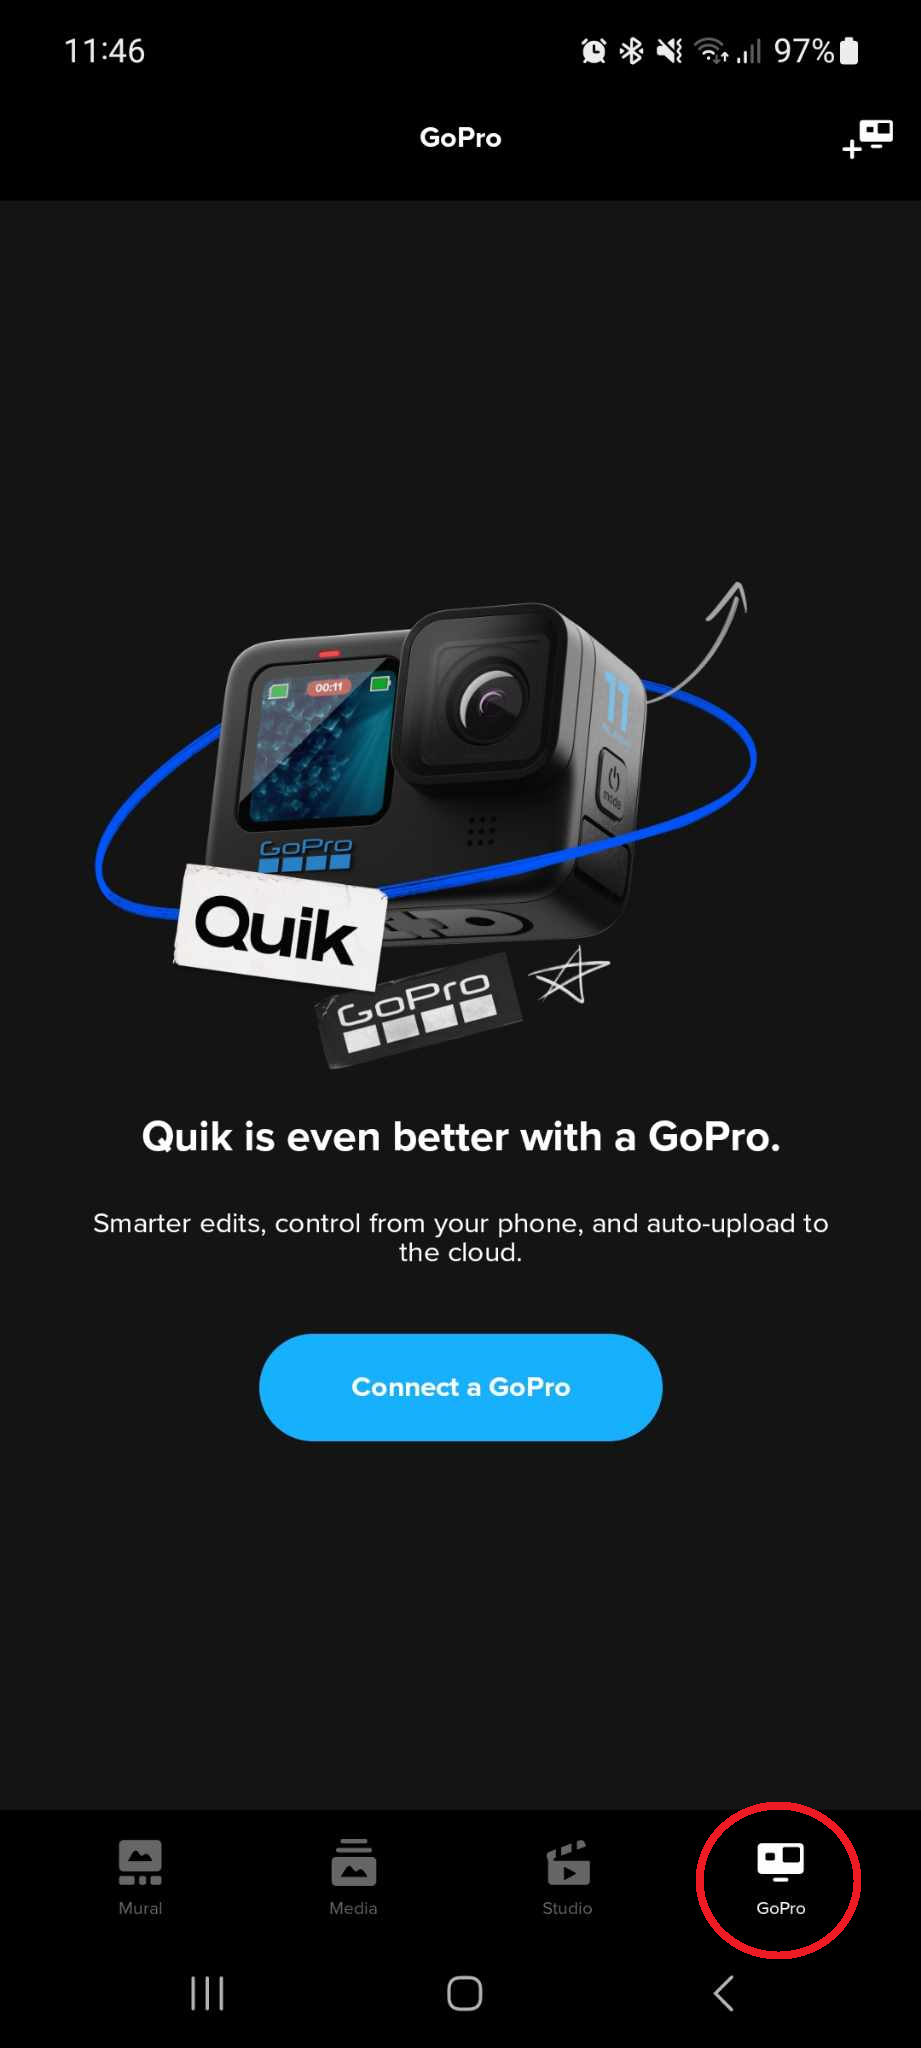
\includegraphics[width=.8\linewidth]{gopro_update1}%
			}		
			\medskip	
		\end{minipage}
		Go to GoPro tab and click Connect a GoPro, choose MAX camera and follow the instructions
		\item If an update is available, the GoPro app will prompt you to update your camera
	\end{itemize}
\end{enumerate}

\chapter{Recording a video}
\section{How to record a video}
\begin{enumerate}
	\item Record a video with your GoPro camera using the following modes:
	\begin{itemize}
		\item Traditional video in HERO or 360 mode
		\item Time Lapse in HERO or 360 mode
	\end{itemize}
	How to use GoPro MAX camera is described in the GoPro MAX manual (link in the introduction). Make sure that you have turned on GPS function otherwise video won't have telemetry data:
	\begin{figure}[H]
		\centering
		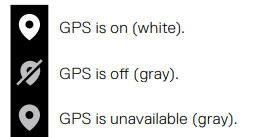
\includegraphics{GoPro_manual_fragment}
		\caption{GoPro Max manual fragment.}
	\end{figure}
	If GPS is off, swipe down to access the Dashboard and Preferences. Click on the Preferences, find option Regional and there turn the GPS On.\\
\end{enumerate}

\section{GoPro video types}
File structure of GoPro Max videos:\\	
GoPro Max creates different types of files during recording, in 360 mode we get:
	\begin{itemize}
		\item .360 file (main video file)
		\item .THM file (thumbnail file)
		\item .LRV file (low-res video file)\\
	\end{itemize}
	In HERO mode (traditional video in 1080p or 1440p) we get:
	\begin{itemize}
		\item .MP4 file (main video file)
		\item .THM file (thumbnail file)
		\item .LRV file (low-res video file)\\
	\end{itemize}
	These files always appear after recording a classical video or a Time Lapse.\\
	
\section{Export camera recordings}
\begin{enumerate}
\item Turn on your GoPro camera.
\item Open your GoPro MAX side panel and connect it to your computer using USB 2.0 to USB-c cable included in a camera set. Information as below should display on the screen:
\begin{figure}[H]
	\centering
	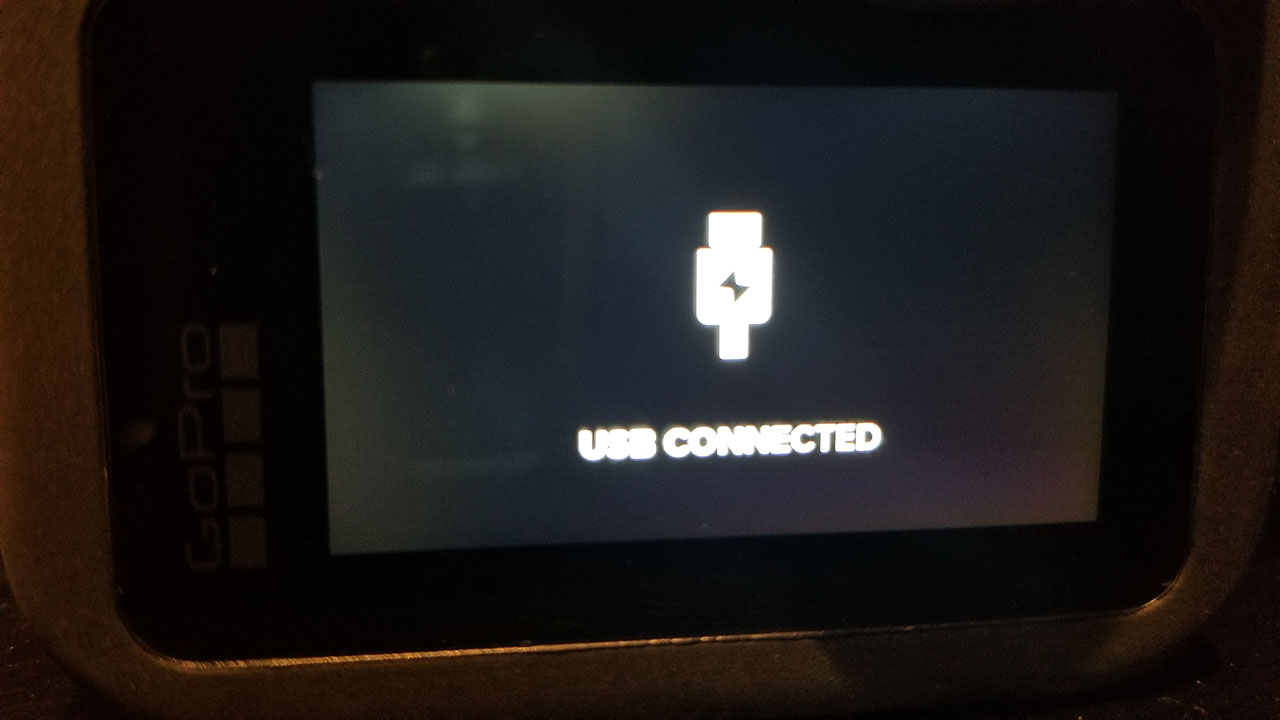
\includegraphics{camera_connected}
	\caption{Successfully connected camera.}
\end{figure} 

\item Now find your connected GoPro camera and navigate through directories:\\

$\textit{GoPro MAX > GoPro MTP Client Disk Volume > DCIM > 100GOPRO}$	\\

Final path should look like this:

\textit{GoPro MAX/GoPro MTP Client Disk Volume/DCIM/100GOPRO}	
\begin{figure}[H]
	\centering
	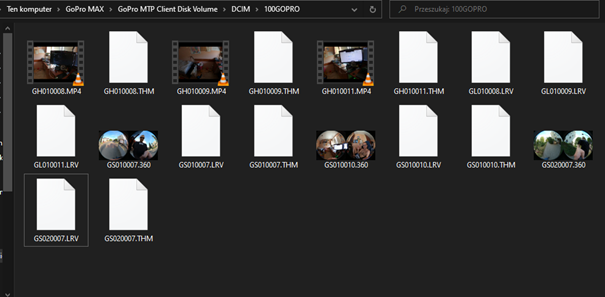
\includegraphics{recording_location}
	\caption{Video files location.}
\end{figure}
\hfill
\item 360 videos’ names and their LRV versions start with GS e.g. GS020007.360, GS020007.LRV.\\

Regular videos’ and their LRV versions’ names start with GH for the former and with GL for the latter e.g. GH010008.MP4, GL010008.LRV. \\
\item Copy videos of your choice and save them on your computer.
\end{enumerate}

\chapter{Install environment and Git}
\section{Install Git}
\begin{enumerate}
	\item Download Git installer from \url{https://gitforwindows.org} and run it.
	\item \begin{minipage}[t]{\linewidth}
		\raggedright
		\adjustbox{valign=t}{%
			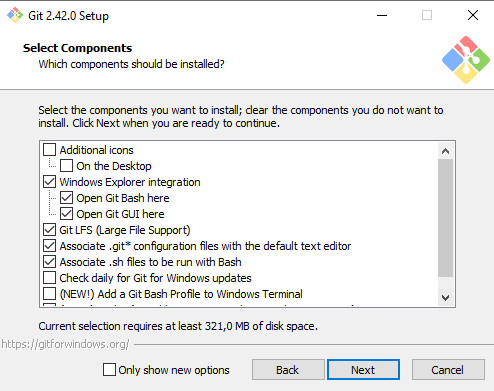
\includegraphics[width=.8\linewidth]{git_install1}%
		}		
		\medskip	
	\end{minipage}
	Select components as seen in the picture above.
	
	\item \begin{minipage}[t]{\linewidth}
		\raggedright
		\adjustbox{valign=t}{%
			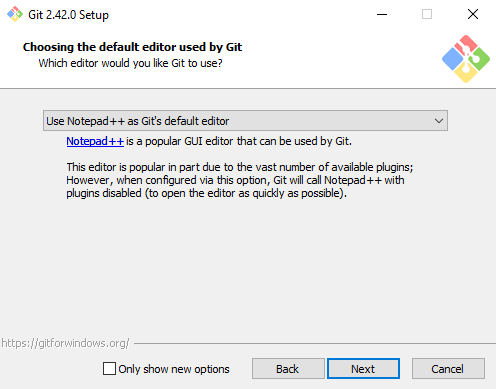
\includegraphics[width=.8\linewidth]{git_install2}%
		}		
		\medskip	
	\end{minipage}
	Choose default editor for Git, I recommend Notepad++ if you don't have it download it from here: \url{https://notepad-plus-plus.org/downloads/}. Install the newest version, you don't have to change anything during installation, just accept and install.
	\item \begin{minipage}[t]{\linewidth}
		\raggedright
		\adjustbox{valign=t}{%
			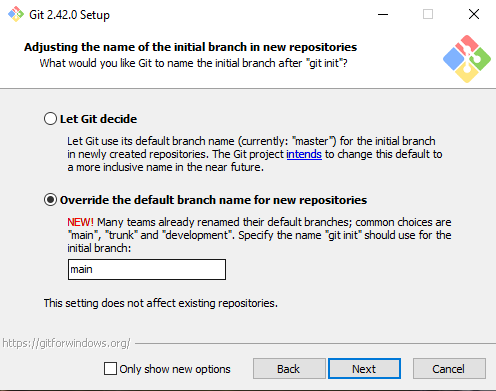
\includegraphics[width=.8\linewidth]{git_install3}%
		}		
		\medskip	
	\end{minipage}
	Select to override since many guides now use the word "main" not "master" for main branch
	\item \begin{minipage}[t]{\linewidth}
		\raggedright
		\adjustbox{valign=t}{%
			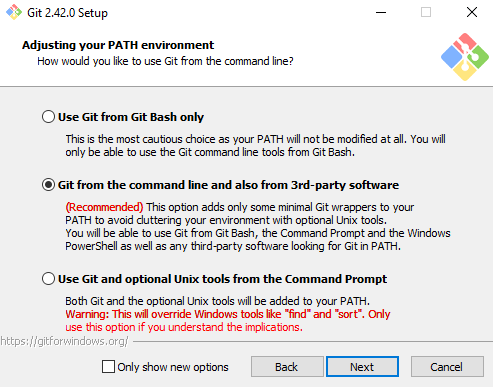
\includegraphics[width=.8\linewidth]{git_install4}%
		}		
		\medskip	
	\end{minipage}
	\item \begin{minipage}[t]{\linewidth}
		\raggedright
		\adjustbox{valign=t}{%
			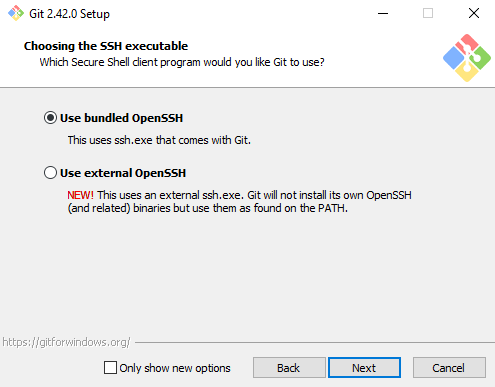
\includegraphics[width=.8\linewidth]{git_install5}%
		}		
		\medskip	
	\end{minipage}
	Choose option to use ssh that comes with Git.
	\item Go through all next appearing windows and change nothing in them. At the end click "Install".
\end{enumerate}
\pagebreak
\section{Install node js}
\begin{enumerate}
	\item Go to \url{https://nodejs.org/en} and download recommended version and run the installer.
	\begin{figure}[H]
		\centering
		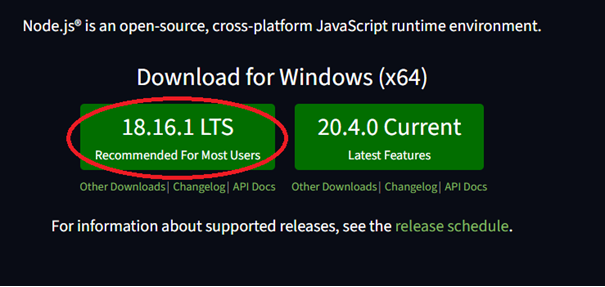
\includegraphics{nodejs_install}
		\caption{Nodejs website fragment.}
	\end{figure}
	\item \begin{minipage}[t]{\linewidth}
		\raggedright
		\adjustbox{valign=t}{%
			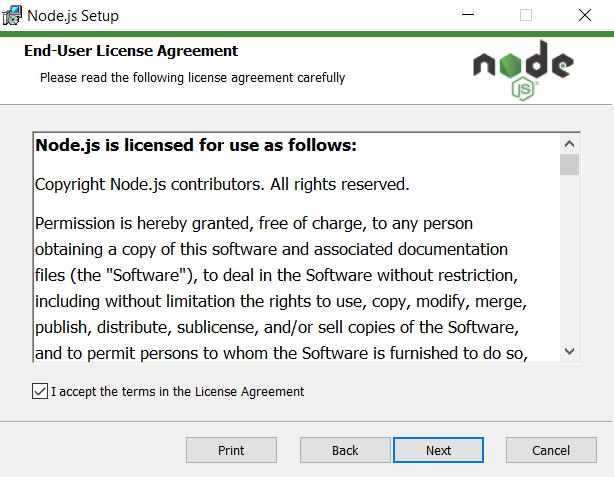
\includegraphics[width=.8\linewidth]{node_install0}%
		}		
		\medskip	
	\end{minipage}
	Accept user agreement
	\item \begin{minipage}[t]{\linewidth}
		\raggedright
		\adjustbox{valign=t}{%
			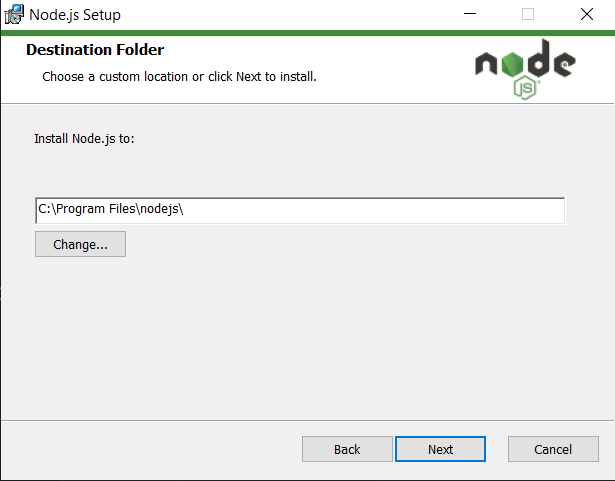
\includegraphics[width=.8\linewidth]{node_install1}%
		}		
		\medskip	
	\end{minipage}
	Choose location, default one is sufficient.
	\item \begin{minipage}[t]{\linewidth}
		\raggedright
		\adjustbox{valign=t}{%
			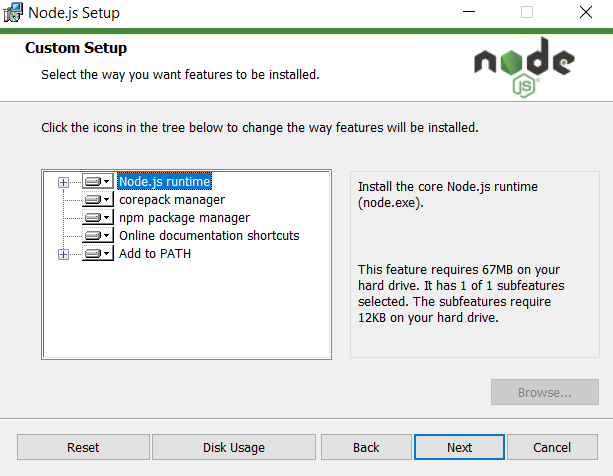
\includegraphics[width=.8\linewidth]{node_install2}%
		}		
		\medskip	
	\end{minipage}
	Do not change anything, install everything as it is.
	\item \begin{minipage}[t]{\linewidth}
		\raggedright
		\adjustbox{valign=t}{%
			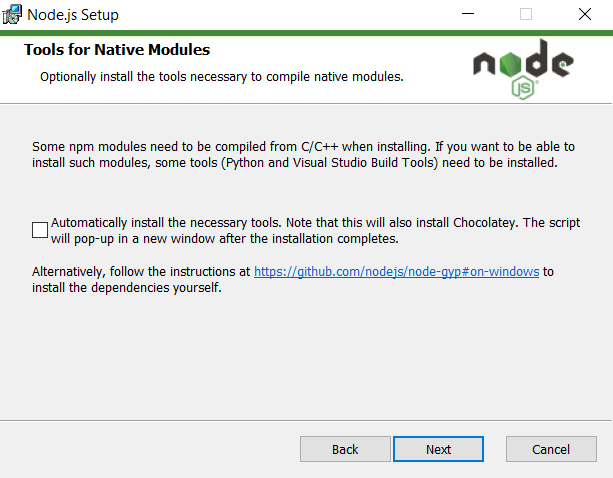
\includegraphics[width=.8\linewidth]{node_install3}%
		}		
		\medskip	
	\end{minipage}
	You do not need to install extra tools to run telemetry extractor.
	\item \begin{minipage}[t]{\linewidth}
		\raggedright
		\adjustbox{valign=t}{%
			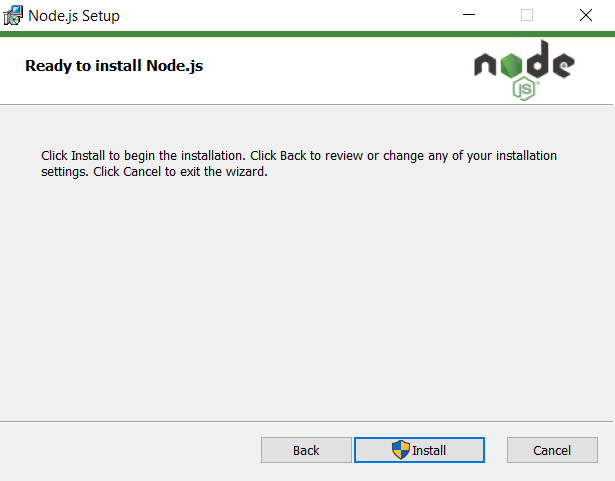
\includegraphics[width=.8\linewidth]{node_install4}%
		}		
		\medskip	
	\end{minipage}
	Click Install to begin installation
	\pagebreak
	\item To check if installed correctly simply open Command Prompt by typing “cmd” in the Start Menu and write “node”, if everything was done properly version of node should appear.
	\begin{figure}[H]
		\centering
		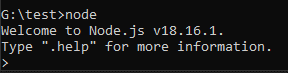
\includegraphics{node_confirmation}
		\caption{Command Prompt fragment confirming proper installation of Nodejs.}
	\end{figure}
\end{enumerate}
After Git and Node js installation it's best to restart your computer, especially if writing "node" in Command Prompt returned error.

\chapter{Run Telemetry-extractor}
\section{Download program and dependencies from Git}
\begin{enumerate}
	\item Download main repository: \url{https://github.com/miloszwojciechowski/Open-vslam-project} and extract it in a directory of your choice.
	\item \begin{minipage}[t]{\linewidth}
		\raggedright
		\adjustbox{valign=t}{%
			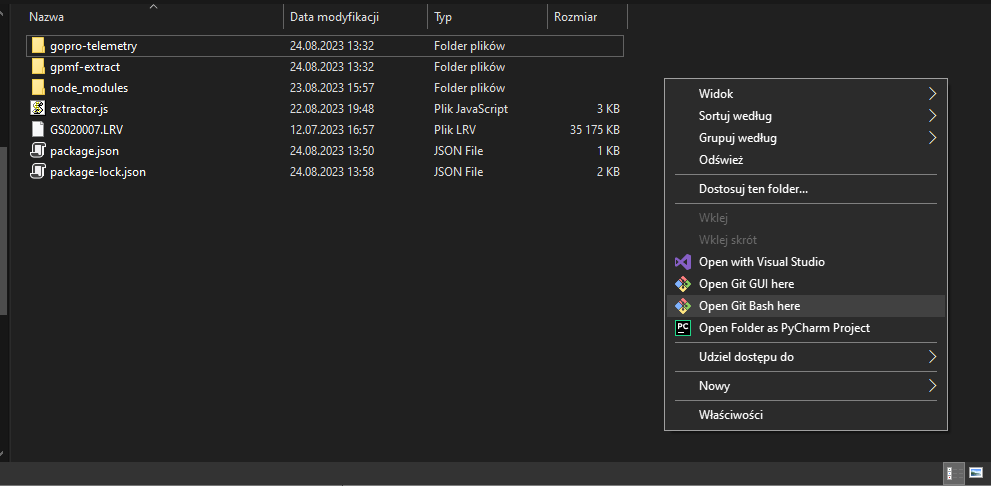
\includegraphics[width=.8\linewidth]{run1}%
		}		
		\medskip	
	\end{minipage}
	Go to folder where the repository has been extracted and right click the on free space and click Open Git Bash here.
	\item \begin{minipage}[t]{\linewidth}
		\raggedright
		\adjustbox{valign=t}{%
			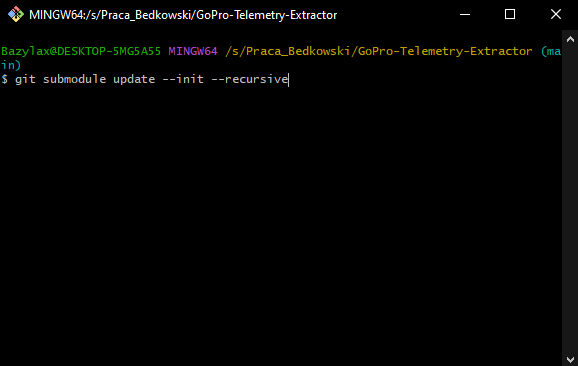
\includegraphics[width=.8\linewidth]{run2}%
		}		
		\medskip	
	\end{minipage}
	Now write the following command: \textit{git submodule update \texttt{-{}-}init \texttt{-{}-}recursive} or copy it from here and right click on the Bash and click Paste. Now run the command. \\
	If you use Git for the first time, information will pop that you need to identify yourself, follow the displayed instructions to log with your GitHub account.\\
	Fulfilling this step will download \href{https://github.com/JuanIrache/gopro-telemetry}{gopro-telemetry} and \href{https://github.com/JuanIrache/gpmf-extract}{gpmf-extract}
	\item You can close git bash and open Command Prompt by typing cmd in Windows Start Menu.
	\item Choose the disc on which you have telemetry extractor by writing disc letter followed by colon e.g. D:
	\item Move to telemetry extractor directory by typing "cd" followed by the name of desired directory e.g cd GoPro-Telemetry-Extractor.
	\item From there move to both: gopro-telemetry and gpmf-extract (again by using cd <directory name>, if you want to go to previous directory type "cd..") and in both directories write \textit{npm install} to install libraries.
\end{enumerate}

\section{Run the program}
\begin{enumerate}
	\item In command prompt either go to GoPro-Telemetry-Extractor location (the one with extractor.js file) or run program from the default place. Telemetry extractor accepts up to 3 arguments:\\
	\begin{itemize}
		\item path to extractor.js (if you went to its location in Command Prompt just write extractor.js e.g "node extractor.js ..."
		\item path to a video file (if a video file is in the same location as the one you are running the script from only a video file name will be needed e.g. you are running script from \verb|S:\GoPro-videos| which contains GS020007.LRV then just write: \\
		" \verb|node S:\GoPro-Telemetry-Extractor\extractor.js GS020007.LRV|..."))
		\item path to location where telemetry csv file should be generated, if not given a default place for it will be extractor.js directory
	\end{itemize}
	\item To extract telemetry use .LRV files if possible since this program won't work for files with size bigger than 2GB
	\item As mentioned above you have a few options to run the program:
	\begin{itemize}
		\item Run from completely random place without extractor.js nor a video file e.g. default Command Prompt directory, command template: \\
		node <extractor.js path> <video file path> <optional telemetry csv generation directory>\\
		e.g.\\
		\verb|node S:\GoPro-Telemetry-Extractor\extractor.js S:\GoPro-videos|\\ \verb|\GS020007.LRV|\\
		
		This will generate telemetry csv file in the extractor.js location.
		\item Run from extractor.js directory that doesn't contain video file, command template:\\
		node extractor.js <video file path> <optional telemetry csv generation directory>\\
		e.g.\\
		\verb|node extractor.js S:\GoPro-videos\GS020007.LRV S:\Telemetry\|\\
		
		This will generate telemetry csv file in \verb|S:\Telemetry\| directory.
		\item Run from directory without extractor.js but with video file, command template:\\
		node <extractor.js path> <video file name> <optional telemetry csv generation directory>\\
		e.g.\\
		\verb|node S:\GoPro-Telemetry-Extractor\extractor.js GS020007.LRV|\\
		
		This will generate telemetry csv file in the extractor.js location.
		\item Run from extractor.js directory containing video file, command template:\\
		node extractor.js <video file name> <optional telemetry csv generation directory>\\
		e.g.\\
		\verb|node extractor.js GS020007.LRV S:\Telemetry\|\\
		This will generate telemetry csv file in \verb|S:\Telemetry\| directory.		
	\end{itemize}
\end{enumerate}
 
\end{document}